\documentclass[10pt,twocolumn,a4paper]{scrartcl}

\usepackage[a4paper,top=3cm,bottom=2cm,left=3cm,right=3cm,marginparwidth=1.75cm]{geometry}
\usepackage{xpatch}
\usepackage[french,english]{babel}
\usepackage[utf8x]{inputenc}
\usepackage[T1]{fontenc}
\usepackage{amsmath}
\usepackage{graphicx}
\usepackage[colorinlistoftodos]{todonotes}
\usepackage[colorlinks=true, allcolors=blue]{hyperref}
\usepackage{float}
\usepackage{tabularx,ragged2e,booktabs,caption}
\usepackage[runin]{abstract}
\usepackage{lipsum}
\usepackage{mathrsfs}
\usepackage{titlesec}



\addtokomafont{disposition}{\rmfamily}

\newlength{\myspace}
\setlength{\myspace}{1em}
\setlength{\abstitleskip}{-\parindent} % make abstract flushleft
\setlength{\absleftindent}{0pt} % make abstract non-indented
\setlength{\absrightindent}{0pt}
\renewcommand{\abstractnamefont}{\normalfont\bfseries} 
\renewcommand{\abstracttextfont}{\normalfont\bfseries} 

\titlespacing\section{0pt}{16pt plus 4pt minus 0pt}{4pt plus 2pt minus 6pt}

\makeatletter
\xpatchcmd{\@maketitle}{\vskip.5em}{\vskip\myspace}{}{}
\makeatother

\makeatletter
\renewenvironment{abstract}{%
    \if@twocolumn
      \section*{\abstractname}%
    \else %% <- here I've removed \small
      \begin{center}%
        {\bfseries \Large\abstractname\vspace{\z@}}%  %% <- here I've added \Large
      \end{center}%
    \fi}
    {\if@twocolumn\else\endquotation\fi}
\makeatother

\setlength{\abstitleskip}{-\parindent} % make abstract flushleft
\setlength{\absleftindent}{0pt} % make abstract non-indented
\setlength{\absrightindent}{0pt}


\title{
%\usefont{OT1}{bch}{b}{n}
\huge Multifidelity Aeroelastic Optimization}
\subtitle{\normalfont \large State-of-the-art bibliographic review \hspace{15mm}QUAGLIA Giovanni}
%\author{}
\date{\vspace{-8ex}}
%\date{May 2019}

\begin{document}

\selectlanguage{english}

\makeatletter
\twocolumn[
   \begin{@twocolumnfalse} 
     \maketitle 
     \begin{abstract}
The reduction of computational time during the aircraft design process in the aerospace industry is a major issue with direct industrial applications \cite{delft}. In the last two decades a strategy named multifidelity has offered significant improvements. This method is based on the combination of models with different accuracy in order to accelerate the analysis. Research on the subject is performed at the mechanical department of ISAE Supaero and at ONERA \cite{Morlier} in a joint effort, the PIR is included in this context. The scope is the development of a more efficient tool able to design an optimized aircraft wing. This paper presents the bibliography study related to the project. The main topics are multifidelity, surrogate models, in particular Kriging interpolation and its derivatives, and more general optimization schemes such as EGO and SEGO. \vspace{15pt}
     \end{abstract}
    \end{@twocolumnfalse}
]
\makeatother

\section{Introduction}
In the last century, complex mathematical models have been developed in order to simulate real systems in many areas of scientific research. The main obstacle to an intensive exploitation of such models, in the process of visualization and analysis, is the computational cost which can easily become prohibitive also for trivial cases \cite{pc}. This problem is even more crucial in the field of aerostructural design, depicted in section \ref{2},  and optimization since many evaluations of the model are required and one single CFD run can demand hours of CPU time. The challenge has been mainly tackled by analyzing surrogate models or meta-models, an approximation of the actual system based on a number of collected samples \cite{Jones2001}. These techniques have their origin in many scientific fields varying from geology and statistics to engineering. A thorough list is beyond the purposes of this work but some examples are Kriging, RBS and Neural Network. Kriging, in particular,as explained in section \ref{3}, is an interpolation method that uses as model a Gaussian process\cite{surrogate}. Different variants, have been efficiently applied to aeroelastic optimization. Nevertheless the actual cost of sampling would still be considerable unless a trade-off between time and accuracy is considered. In recent years multifidelity, detailed in section \ref{4}, has been proposed as a valuable strategy to reduce computational time. Under such approach the results employed to train and enrich the model derive from sources of different precision and are mixed in order to reduce the overall cost. These sources can be seen as black-box functions as explained in \cite{bbf} and are connected in an optimization environment section \ref{5}.\\ Finally the objective of the PIR is presented in section \ref{6}.

\section{Aerostructural problem}\label{2}
The context of the optimization is the aeroelastic problem. In literature, two approaches to solve it can be found, the monolithic and the partitioned. The latter is the most applied nowadays and it consists in the coupling of two different solvers for the structural and fluid problems such as a FEM and a CFD software. The theory is reported with the notation used in \cite{delft}.

\begin{equation*}
    \mathbf{y} = \mathcal{F} (\mathbf{x}), \hspace{0.5 cm} \mathbf{x} = \mathscr{S} (\mathbf{y})
\end{equation*}


\noindent Here, \mathbf{x} and \mathbf{y} are the vectors containing the structural and aerodynamic variables, namely the nodes displacements and the fluid pressure along the airfoil. \mathscr{S} and \mathcal{F} are the structural and fluid problems. The coupling can be expressed as:

\begin{equation*}
    \mathbf{x}^* = \arg \min_{\mathbf{x} \in \rm I\!R ^{N^{s}}} \mid \mid \mathcal{R} (\mathbf{x}) \mid \mid
\end{equation*}

\begin{equation*}
  with \hspace{0.5 cm} \mathcal{R}(\mathbf{x}) = \mathscr{S} \circ \mathcal{F} (\mathbf{x}) - \mathbf{x}
\end{equation*}

\noindent The solution must be found iterating but the algorithm is then treated as a black-box function which provides the converged solution and all the quantities of interest (QoI) to be constrained or optimized.

\section{Surrogate Models}\label{3}
In this section it is first explained how to create a surrogate model through Kriging interpolation according to \cite{Jones2001}, then the Co-Kriging is introduced. The method was invented by D.G. Krige in the field of mineral extraction and later developed by G. Matheron. Given a set of evaluations $\mathbf{y}_i(\mathbf{x}_i)$, it defines the predictor that minimizes the expected squared prediction error subject to: being unbiased and, being a linear function of the observed $\mathbf{y}_i$’s. The process is modeled as a random variable $\mathbf{Y(x)}$ with mean $\mu$ and variance $\sigma^2$ and the covariance function is approximated as:

\begin{equation*}
Corr[\mathbf{Y(x}_i),\mathbf{Y(x}_j)] = exp(-\sum_{l=1}^{d}\theta_l \mid \mathbf{x}_{il}-\mathbf{x}_{jl} \mid^{p_l})
\end{equation*}

\noindent The parameters $\mu$, $\sigma^2$, $\theta_l$ and $p_l$ are tuned using the samples and maximizing the likelihood function usually with a Genetic Algorithm but the size of this problem can easily become demanding. As a solution parameters are not always updated or the choice $p = 2$ is often made \cite{}. Finally the predictor for an unknown additional sample is:

\begin{equation*}
\mathbf{\hat{y}(x)} = \hat{\mu} + r^{'}R^{-1}(\mathbf{y}-1\hat{\mu})
\end{equation*}

\noindent Where $r$ and $R$ contain the covariances of the samples and are functions of the parameters.
\\This method is extremely useful because it provides a prediction of the function in a new point in the design space along with its uncertainty based on the Gaussian process used. The possible deviation is zero in the already known points and increases moving away from them.% as it can be seen in figure 1.

%\begin{figure}[H]
%  \centering
% 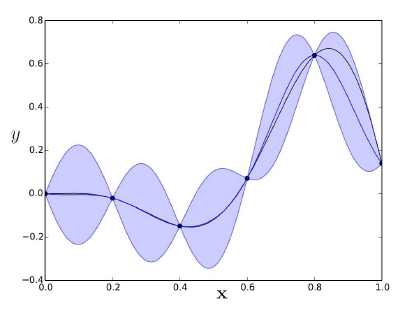
\includegraphics[width=0.5\textwidth]{Kriging.png}
%  \caption{Example of Kriging interpolation. \textit{Taken from \cite{}}}
%\end{figure}

\noindent Co-Kriging \cite{surrogate}, is an extension of this method in the case where values $\mathbf{y}_i$ come from two sources, the first more precise, high fidelity, and the other less, low fidelity. The model builds the predictor in the same fashion but considering also a random variable for the difference between the sources. This meta-model is fundamental as it is shown in the next section. Finally literature provides many improvements to tackle problems such as noisy data \cite{surrogate}, parameters tuning time and ill conditioned functions \cite{bbf}, offering a variety of meta models to be used in optimization environments \cite{MF} \cite{RBF}. 

\section{Multifidelity}\label{4}
The concept of multifidelity has already been introduced, the space of possible sources is huge. Samples used to train the model could come from experiments, software of different levels of modelling such as CFD or panels in aerodynamics, a coarse and a fine mesh on the same problem or even a change in the convergence criteria for an iterative algorithm \cite{delft}. In the conducted research two levels of fidelity are used in the form of black-box aeroelastic solvers. The HF is the coupling of the CFD software ADFlow with a fine meshed Nastran model while the LF model uses the panel method implemented in Panair and a coarser structural mesh.\\

\section{Optimization}\label{5}
Optimization is performed in the SEGO framework explained in \cite{Morlier}. First a sampling campaign collects HF and LF points to create a Co-Kriging model. Then the algorithm chooses the next variables design at maximum of the Expected Improvement (EI) defined as:

\begin{equation*}
E[I(\mathbf{x})] = E[max(f_{min},0)]
\end{equation*} 

\noindent In this approach the minimum already found and the uncertainty on the remaining regions given by the interpolated stochastic model are balanced. The result is a combination of exploration and exploitation of the design space. Computing the maximum of the EI is not trivial, even if the function is shown to be monotone with respect to $\mathbf{y}$ and $\sigma$ in \cite{bbf}, and a large part of research addresses this problem \cite{Morlier},\cite{}.\\
The SuperEGO implementation uses a slightly different criteria called WB2 and includes also functional constraints. Moreover, respecting MF, each new point can be computed according to a cost-weighting-criteria using HF or LF in order to preserve computational time.

\section{Future work}\label{6}
In this brief overview, the main research subjects merging in multifidelity aeroelastic optimization have been presented. During the PIR, the first task to be handled is the realization of the coarse meshed Nastran model. The LF and HF boxes currently uses the same structural model, mining the possible results of multifidelity. Later it will be possible to improve the existing SEGO framework according to some cues found in the bibliography study.

\onecolumn{
\bibliographystyle{apalike}
\bibliography{ref}}

\end{document}
